% Gemini theme
% https://github.com/anishathalye/gemini

\documentclass[final,20pt]{beamer}

% ====================
% Packages
% ====================

\usepackage[T1]{fontenc}
\usepackage{lmodern}
\usepackage[orientation=portrait,size=a0,scale=1.05]{beamerposter}
\usetheme{gemini}
\usecolortheme{labsix}
\usepackage{graphicx}
\usepackage{booktabs}
\usepackage{tikz}
\usepackage{pgfplots}

\usepackage{caption}
%\captionsetup[subfigure]{labelformat=empty}
 

% ====================
% Lengths
% ====================

% If you have N columns, choose \sepwidth and \colwidth such that
% (N+1)*\sepwidth + N*\colwidth = \paperwidth
\newlength{\sepwidth}
\newlength{\colwidth}
\setlength{\sepwidth}{0.04\paperwidth}
\setlength{\colwidth}{0.44\paperwidth}

\newcommand{\separatorcolumn}{\begin{column}{\sepwidth}\end{column}}

% ====================
% Title
% ====================

\title{Mutation Accumulation in an Asexual Relative of Arabidopsis}

\author{John T.Lovell \inst{1} \and Robert J. Williamson \inst{2} \and \textit{et al.}}

\institute[shortinst]{\inst{1}  Dpt. of Integrative Biology, University of Texas at Austin, USA
\samelineand \inst{2} Dpt. of Ecology and Evolutionary Biology, University of Toronto, Canada
}

% ====================
% Body
% ====================

\begin{document}

\begin{frame}[t]

  
  \begin{alertblock}{Asexual reproduction}
    {\Large 
    Asexual reproduction circumvents the many costs associated with sex, such as 
    finding and attracting mates. However, the most prominent reproduction mode 
    among multicellular organisms is sex. 
    %Within finite populations,
      \begin{itemize}
        \item \textbf{sexual recombination 
        increases the probability of fixing beneficial mutations} through Hill-Robertson 
        effect.
        \item \textbf{stochastic loss of conserved alleles}, a process known as Muller's Ratchet, occurs more frequently
        in lineages that don't undergo sex
      \end{itemize}
     %Furthermore, .\hfill

    $\Rightarrow$ \emph{Both processes lead to an increased rate of deleterious mutation accumulation 
    in asexual lineages.}
    \hfill}
  \end{alertblock}

  \begin{columns}[t]
    \separatorcolumn
    \begin{column}{\colwidth}
  \begin{block}{Case study : sympatric populations of \textit{Boechera spatifolia}}
    \textbf{Apomixis} is an asexual reproduction mode via seeds.\\ It is common (> 30\%) 
    within the genus \textit{Boechera} and appears to be an ancient characteristic of the genus.
    \begin{figure}

      \begin{minipage}[c]{0.67\textwidth}
      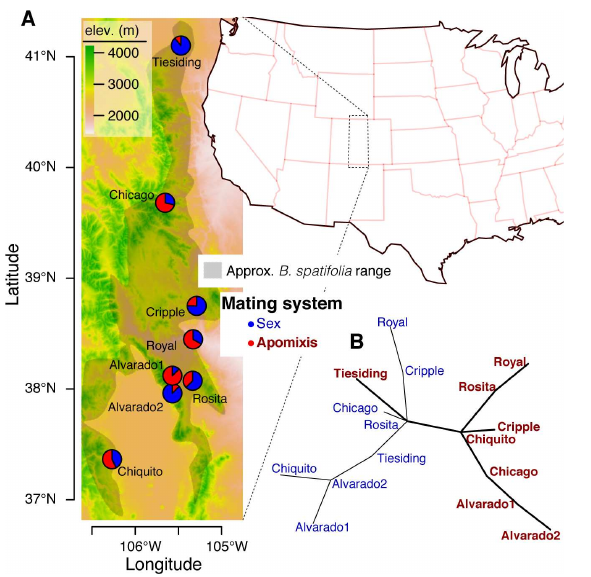
\includegraphics[width=\textwidth]{./fig1.png}
      \end{minipage}\hfill
      \begin{minipage}[c]{0.3\textwidth}
      \caption{(\textbf{A}) Geographic locations of sympatric sample populations 
      where the proportions of {\color{blue}\textbf{sexual}} and
      {\color{red}\textbf{apomictic}} individuals screened are indicated. 
      SNP data from one individual per mating system per population were used to 
      generate a minimum spanning network where edge length is proportional to genetic
      distance (\textbf{B})}.
      \end{minipage}
    \end{figure}

  \end{block}

  \begin{block}{Apomicts show increased sequence diversity and heterozygosity}
    \begin{itemize}
      \item Sexual \textit{B. spatifolia} are self-compatible and highly inbred
      \item across all sites and populations, 
      \textbf{apomicts displayed much greater observed heterozygosity than sexuals}
      \item such elevated heterozygosity may be due to the \textbf{accumulation of mutations in
      the non-recombining apomictic genomes}, in the absence of gene conversion
    \end{itemize}
    
    \begin{figure}
      %\begin{minipage}[c]{0.67\textwidth}
      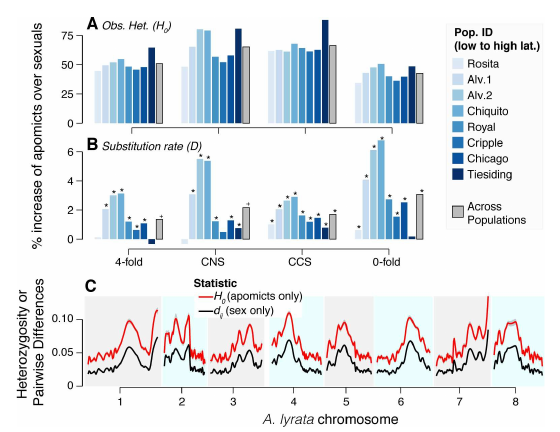
\includegraphics[width=\textwidth]{./fig2.png}
      %\end{minipage}\hfill
      %\begin{minipage}[c]{0.3\textwidth}
      \caption{(\textbf{A}) Observed heterozygosity (all significant) and (\textbf{B}) substitution rate 
      (Fisher's test $P \leq 0.05^*, P \leq 0.1^+$) increase 
      percentages, in apomictic populations. \\
      (\textbf{C}) Heterozygosity of each apomictic
      genotype and proportion of pairwise differences between each sexual genotype ($d_{ij}$) were calculated for non-
      overlapping 20k SNP windows.
      }
      %\end{minipage}
      
    \end{figure}
  \end{block}
  \vfill
  \small{Louis Duchemin M2 Bioinfo -- 2018/2019}
\end{column}

\separatorcolumn

\begin{column}{\colwidth}
  \begin{block}{Hybrid origin of apomictic lineages}
    To determine whether apomictic haplotypes were derived solely from \textit{B. spatifolia} (non-hybrid origin) 
    or from hybridization with another \textit{Boechera} species, 
    22k trees generated from 5-sequence haplotype alignments were classified into six possible topologies.

    \begin{figure}
      \begin{minipage}[c]{0.67\textwidth}
        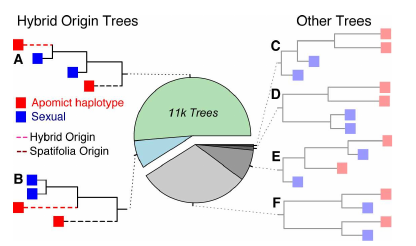
\includegraphics[width=\textwidth]{./fig3.png}
      \end{minipage}\hfill
      \begin{minipage}[c]{0.3\textwidth}
      \caption{\textbf{Classification of haplotype trees to infer the impact of hybridization.} 
      Those trees that present a hybrid evolutionary history are plotted on the left (\textbf{A-B}), 
      while all other threes are on the right (\textbf{C-F}).
      All trees are rooted against \textit{A. lyrata} as external group.
      }
      \end{minipage}
    \end{figure}
    \begin{itemize}
      \item Topologies where one apomictic haplotype was
      basal while the other was nested within the sexual haplotypes indicated a
      hybrid origin. 
      \item Topologies producing apomictic haplotypes diverging from basal sexual 
      sequences are in favor of a true breeding origin.
    \end{itemize} 
    \textbf{The bulk (59.0\%) of the trees had a topology indicative of a hybrid origin. }

    % increased apomictic heterozygosity and
%the observation that 5/6 unambiguous trees were of hybrid origin, provide strong evidence that
%B. spatifolia apomicts were originally derived from hybridization.


  \end{block}

  \begin{alertblock}{Apomicts harbor more deleterious mutations than sexuals}

    \begin{figure}
      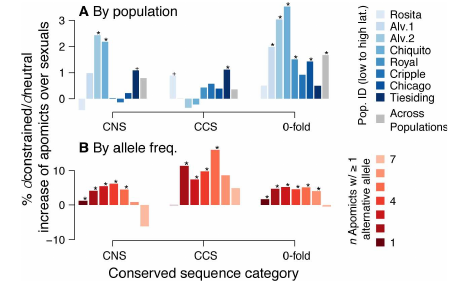
\includegraphics[width=\textwidth]{./fig4.png}
      \caption{\textbf{Signatures of relaxed purifying selection in apomicts.}
      $\frac{d_N}{d_S}$ ratios were calculated for each population (\textbf{A}) and each SNPs 
      binned by their derived allele frequency among the 7 southern apomictic genotypes (\textbf{B}).
      For example n = 1 indicates a site where a single apomictic genotype has a derived allele, while n = 7
      represents sites where all apomicts share a derived allele.
      }
    \end{figure}

    \begin{itemize}
      \item \textbf{Deleterious mutations are fixed at an accelerated rate in asexual 
      populations due to the absence of recombination.}
      \item \textbf{Efficiency of purifying selection is decreased in apomictic lineages}
      \item \textbf{Apomicts accumulate mutations in otherwise conserved sites, 
      consistently with the predictions of Hill-Robertson interference and Muller’s
      Ratchet.}
    \end{itemize}
    
%      Combined, our data demonstrated two levels of genome sequence diver-
% gence between Boechera mating systems. As expected, divergence was driven primarily by
% hybridization, as this is the mechanism through which apomixis spreads. However, contempo-
% rary mutation accumulation also impacted the molecular evolution of apomicts. In particular,
% these results demonstrated that apomicts were accumulating mutations in otherwise conserved
% sites, a pattern consistent with the predictions of 

  \end{alertblock}

  \begin{block}{\large References}

    \nocite{*}
    \footnotesize{\bibliographystyle{plain}\bibliography{poster}}

  \end{block}


\end{column}

\separatorcolumn
\end{columns}
\end{frame}

\end{document}
